\documentclass{article}

\usepackage {amsmath}
\usepackage {textcomp}
\usepackage {setspace}
\usepackage [pdftex]{graphicx}
\usepackage[sort&compress]{achemso}
\usepackage{lineno}

\usepackage[
top    = 0.5in,
bottom = 1.0in]{geometry}
%left   = 2.50cm,
%right  = 2.50cm]{geometry}

% some formatting tags
%\oddsidemargin  0.0in
%\evensidemargin 0.0in
%\textwidth      6.5in

\title{Dancing on Water: The Choreography of Sulfur Dioxide Adsorption to Aqueous Surfaces}
\author{Eric S. Shamay \and Kevin E. Johnson \and Geraldine L. Richmond}

\begin{document}


\newcommand{\suldiox}{SO$_2$}
\newcommand{\ang}{\,$\textrm{\AA}$}
\newcommand{\angs}{\ang}
\newcommand{\wat}{H$_2$O}
%\newcommand{\deg}{$\,^{\circ}$}

\maketitle

%\onehalfspacing
\linenumbers 
\doublespacing


\begin{abstract}
One might expect the high surface tension of water to be a barrier to adsorption of a gas into the liquid phase, but we know that gaseous adsorption on and into a water surface is a common phenomenon on this planet.  What is not commonly known is how an atmospheric gas such as \suldiox~and molecules at the water surface can overcome the barrier created by strong water-water surface bonding interactions.  What this interplay looks like, the distances from the water surface at which these attractive interactions begin, and how they influence the orientational nature of both \suldiox~and surface water molecules is the focus of this computational study.  The results fill a void in the information about this system existing from previous experimental studies by providing information about the dimensional nature of the gas-surface interactions, and the details of how the two species twist and turn orientationally with increased surface interactions.  Classical molecular dynamics have been employed in both equilibrium and steered molecular dynamics (SMD) simulations for \suldiox~at a neat-water surface, and at a surface with high interfacial \suldiox~concentrations.  The results provide new molecular insights for understanding the interaction of this prevalent gas on aerosols and other aqueous surfaces in the environment.
\end{abstract}

\section{Introduction}

Our current molecular-level understanding of adsorption phenomena relies on experiments and theory of model systems, and on an increasing number of computational simulations of molecular processes. What species form during gas adsorption onto liquid surfaces, and what are the intermediary steps? To what extent does an adsorbing gas affect liquid water surface molecules, or the structure of the interface throughout an adsorption process? Are specific gas or liquid molecular orientations necessary for gaseous adsorption? Very little work has been done to characterize the molecular processes that take place during the transit of a molecule from the gas phase onto a liquid interfacial region. Furthermore, experiment does not yet provide us with the resolution necessary to determine the geometries of adsorbing gases, or to determine the orientations of the molecules at the liquid surface near the adsorption site. In this work we look at the orientational properties of sulfur dioxide gas adsorbing to a water surface as a model for the transit of gases on to liquid interfaces.

The interactions between sulfur species and aqueous systems are currently an active area of chemical research. Sulfur dioxide enters the environment as an important industrial product, and also naturally through terrestrial processes. Atmospheric dust particles and gases have been implicated in the oxidation of \suldiox, and act as reaction surfaces for chemical mechanisms that are still poorly understood.\cite{Baltrusaitis2011,Rubasinghege2010,Li2007} \suldiox~acts as a major component of atmospheric pollution, and is a precursor to acid rain formation, and cloud nucleation. Its high solubility in water makes \suldiox~an integral compound in many aqueous atmospheric reactions, as well. We seek a fuller understanding of the interactions between \suldiox~and water at interfaces because they are central to many atmospheric particle and aerosol reactions.

Our recent vibational sum frequency spectroscopy (vsfs) experiments provided insight into the adsorption and reaction of gases in atmospheric aerosols.\cite{Tarbuck2005,Tarbuck2006} We concluded that an \suldiox~surface hydrate complex forms when an aqueous surface is exposed to \suldiox~gas. A computational study by Baer et al.\cite{Baer2010} then made a series of predictions of the specific nature of the hydrated complex through classical and ab initio simulations. That work developed a detailed picture of the nature of the \suldiox~surface complex with water, and related it to the surface water OH vibrational IR spectra.

Our latest vsfs experiments on \suldiox~behavior further expand our understanding of \suldiox~in atmospheric processes.\cite{Ota2011} A temperature study showed that the binding of gaseous \suldiox~to water surfaces is greatly enhanced at atmospherically relevant cold temperatures. The surface binding of unreacted \suldiox~complexes was found to be a completely reversible process. The same study also showed that low pH aqueous environments inhibit the bulk reaction of \suldiox, but do not affect the surface binding of the gas molecules. The resultant experimental spectra suggest that the surface waters reorient in response to the presence of adsorbed \suldiox. Knowing that reorientation may occur due to \suldiox~adsorption, how can we confirm it? what is the nature of the reorienting waters? How do they reorient, and to what extent? Conclusive experimental evidence of the adsorbing gas or surface water molecular orientation is still missing, so we are moved to use computational methods for further understanding this phenomena.

In this study we look at computed orientational depth profiles of water and \suldiox~before and after the adsorption process. Spectroscopic experiments can not probe depth or orientation profiles of surface species in the same detailed manner as computational simulations. We determine the effect of introducing \suldiox~to a \wat~surface, and analyze the orientational response of both the \suldiox~and \wat~molecules using equilibrium and steered (SMD) classical molecular dynamics simulations. We use a technique of steering a gas molecule into the aqueous phase, and characterize the transit through the interfacial region. This unique method gives us much greater insight into the behaviors of gas molecules as they move near to liquid water. We also simulate the behavior of adsorbed \suldiox~at equilibrium to show how an already-adsorbed \suldiox~behaves on a water surface. The results of this study will help us to understand the behavior of adsorbing gases. Computational simulations like this are necessary to further understand the microscopic nature of the gaseous adsorption process, as many of the molecular-level subtleties are lost in experiment. Along with other ongoing experiments and computations, we develop a more complete picture of gaseous adsorption on aqueous surfaces.

\section{Computational Approach}

Molecular dynamics simulations were performed using the Amber 11 software suite.\cite{Case2010} Polarizable models for the \wat~and \suldiox~molecules were used in the simulations, and have been used previously in studies on interfacial systems because they are known to more accurately reproduce interfacial structure and free energy profiles.\cite{Wick2007,Rivera2006,Dang1998} The \wat~model used is the POL3 water model (also discussed in the supplemental information),\cite{Caldwell1995} and for \suldiox~we used the model of Baer et al. that places a single polarizable center on the sulfur atom.\cite{Baer2010} An intermolecular cutoff of 12\angs~was used for long-range electrostatic forces. The simulations were performed in the NVT ensemble using Langevin dynamics for temperature control. Induced dipoles were treated by the polarizable potential functions of the Amber molecular dynamics software.

All simulations began with an equilibrated cube of 900 \wat~molecules, with sides of length 30\angs. The long axis of each simulation cell (the axis normal to the water surface) was then lengthened to 120\angs, and the systems were further equilibrated for 10 ns. The simulations all employed periodic boundaries to create an ``infinite-slab'' geometry. After equilibrating the neat-\wat~slabs two types of systems were created by introducing \suldiox: a single-\suldiox~system, herein referred to as the ``neat-water'' system, and a ``saturated'' \suldiox~system with many gaseous surface and bulk-water \suldiox~molecules.

The low and high concentration simulated systems, ``neat-water'' and ``saturated'', respectively, were created as follows: the neat-water simulation involved the addition of a single \suldiox~molecule either within the bulk of the water slab (for equilibrium MD), or above the slab surface (in the SMD simulations). The single-\suldiox~neat-water system was then evolved for 2 ns to produce an equilibrated starting configuration. Because of the extremely low concentration of \suldiox~in the neat-water system the surface waters behave similarly to a true neat-water air-liquid interface. The neat-water system orientational results shown later in this work reproduce well the results of our previous orientational studies of surface water behavior.\cite{Walker2006b,Hore2008} The saturated system had 22 \suldiox~molecules introduced to the water slab bulk in order to saturate it to a level coinciding with the Henry's law constant for \suldiox~in water (k\textdegree$_H = 1.4$ mol/kg*bar).\cite{Lide2000} Additionally, 50 \suldiox~molecules were introduced into the gas phase outside of the saturated water slab to simulate an added \suldiox~gas pressure. The additional gas in the vapor phase was added over the course of several ns to keep a constant 1 atm of \suldiox~pressure above the water surface as \suldiox~gas molecules adsorbed to the surface. The saturated system with both bulk and gaseous \suldiox~was then evolved for 2 ns to produce a starting configuration for further saturated simulations.

\subsection{Equilibrium Molecular Dynamics Simulations}

Equilibrium simulations involved adding \suldiox~to a water slab and equilibrating as outlined above. The neat-water system had a single \suldiox~added to the center of the water box, representing a concentration of 0.06 M. The more concentrated ``saturated'' system consisted of 22 \suldiox~molecules in the bulk corresponding to a concentration 1.35 M. This saturated system was exposed to an additional 50 \suldiox~in the gas phase above the water surface. After equilibration for 2 ns, both the low and high concentration systems were then evolved for a further 10 ns data collection using a time step of 0.5 fs, with atomic coordinates recorded every 100 fs.

\subsection{Steered Molecular Dynamics Simulations}

% need to add in the specifics about the SMD routine, force constants, calculations, etc.
A second set of simulations began with an equilibrated water slab as in the surface equilibrated method above. However, in both the neat-water and saturated starting systems, a single \suldiox~was introduced 20\angs~above the water slab surface, with the sulfur atom tethered to its initial position. The systems were then evolved for 1 ns, taking coordinate snapshots every 20 ps to create 50 starting points for further simulations. Steered molecular dynamics (SMD) were then performed on the 50 system configurations (in both the neat-water and saturated configurations) to guide the \suldiox~down towards a tethered water near the water slab's center of mass by applying a small steering force to the \suldiox-sulfur atom. This steering technique has been previously developed and used to successfully model chemical events.\cite{Isralewitz2001,Giorgino2011,Bizzarri2011,Strzelecki2009,Patargias2009,Liu2006} The \suldiox~thus passed through the continuum of environments from gas phase to (neat- and saturated) water surface adsorption, and finally absorption into the bulk of the \wat~slab. Each of the SMD simulations were performed for a total of 200 ps, using a time step of 1 fs, and taking snapshots of the system every 25 fs. Figure \ref{fig:starting-configurations} illustrates two sample starting configurations for the SMD simulations, showing both the neat-water slab and the saturated slab configurations before steering the \suldiox~towards the water bulk.

A separate set of SMD simulations were performed with tethering of one of the \suldiox-oxygens to the water slab center of mass. This was done to ensure that the orientation of the \suldiox~during the adsorption transit was not an artifact of the choice of atom used for tethering. The simulations produced the same results (not shown) for the orientational analyses, so the data from the original tethering scheme was used.

\begin{figure}[h!]
	\begin{center}
		\includegraphics[scale=1.0]{images/startingconfigurations.png}
		\caption{Sample starting configurations for the two types of SMD simulations. The neat-water slab simulation introduces a single \suldiox~molecule that is then guided into the surface of the water and further into the bulk (left). The saturated slab simulation begins with a water system that has been loaded with \suldiox~to saturate the water phase, and also with a high pressure of \suldiox~gas (right). The single \suldiox~(shown at the top) is then steered through the surface region saturated with \suldiox~molecules, and into the water bulk.}
		\label{fig:starting-configurations}
	\end{center}
\end{figure}

\subsection {Aqueous Surface Location}

	The first portion of the studies involved creating orientational depth-profiles in the interfacial region comprised of \suldiox~and \wat~upon exposure and adsorption of the gas. Recognizing that a liquid surface is a dynamic boundary that is neither flat nor stationary, we must define a reference point in the interfacial region which we refer to here as the water surface location. Several previous studies have used the technique of fitting a line shape to the averaged density profile of the water, and extracting interfacial shape and location parameters to define the water surface location.\cite{Shamay2010,Wick2006c,Chowdhary2006} Hyperbolic tangent functions have been used often, and values for the ``Gibb's dividing surface'' location, and interfacial width have thus been determined.\cite{Matsumoto1988} However, in long simulations the location and shape of the interface changes, and the motion of surface waters alters the interfacial width at any given time step. Thus, the density profile fitting will capture averaged widths and locations, not instantaneous values. Similarly, the averaged values of location and width will obscure information about any drift or deformations the surface undergoes. The analysis presented here attempts to retain these subtleties through the use of a ``corrected'' coordinate system.
	
Figure \ref{fig:density-flaw} demonstrates the problem of surface location drift during a simulation (even with utilizing the Amber NSCM parameter). Figure \ref{fig:density-flaw}A shows the density profile of water and \suldiox~over the course of one of the 10 ns trajectories used in this work using the original uncorrected coordinates of the system taken from the raw atomic positions of the molecular dynamics data output. The water density profile and location (thin gray line in Figure \ref{fig:density-flaw}A) is produced by averaging the instantaneous density profile at each time step in the simulation over all the time steps. The water profile was then fit to a $\tanh$ function (black line) to extract the position and width parameters of the water surface. The fitted surface water density profile has a width of 3.77\angs, which is comparable to values reported for similar neat-water systems.\cite{Dang1997,Hore2008} A bulge in the gas-phase ($\leq 52$\angs) side of the water density profile is indicative of the drift of the water slab over the course of the trajectory. Thus the calculated location and width from the $\tanh$ line fit are not accurate over long trajectories for defining a stationary reference point. 

	To overcome this problem we define the water surface location by calculating a reference location at each time step by averaging the positions of the waters contained in the topmost monolayer. This provides a consistent and intuitive reference point in the simulations to which we relate our analyses, but does not increase the computational burden. The number of waters included in the averaging is determined by taking a few issues into account. First, counting the waters found in the topmost cross-section of the water slab over several time steps indicated between 65-75 waters that established a full monolayer. This was done by a visual inspection of the slab using the VMD MD visualization package.\cite{Humphrey1996} Alternatively, assuming a spherical model of water with a radius of 2.2\angs, two layers of hexagonally tight-packed spheres yielded a similar number of surface water molecules. Increasing the number of waters used in calculating the surface location diminishes the effects of the few waters that briefly rise above the surface into the gas phase, stabilizing both the surface position and thickness values. Taking the close-packed model as a maximum number of waters fit into a flat surface, the topmost 70 water molecules were used for calculating instantaneous water surface locations for each simulation step. 
  
This method for finding the outer monolayer location was implemented, and the surface location is plotted as a function of simulation time in Figure \ref{fig:density-flaw}B. It is apparent from the surface location plot that the water slab location, and thus the surface location, drifts over the 10 ns, spanning approximately 12 \angs. However, the maximum standard deviation of the positions of the waters comprising the surface layer at each time step is only 1.85 \angs. Consequently, all depth locations in our analyses are calculated relative to the instantaneous surface location at the corresponding time step of the trajectories.

\begin{figure}[h!]
	\begin{center}
		\includegraphics[scale=1.0]{images/density/density-location.png}
		\caption{(A) Density profiles of \wat~(Gray) and \suldiox~(red) from a 10 ns simulation of the neat-water system with a single sulfur dioxide. The \wat~density profile was fit using a hyperbolic tangent function (black) to extract location and width data for the water surface. Position values are based on the atomic position data of the water oxygens and \suldiox~sulfurs from the raw molecular dynamics output. (B) The instantaneous location of the outer \wat~monolayer was calculated for each simulation time step (blue), and the surface location extracted from the density fitting was also shown for reference (horizontal dashed line). Long simulations of liquid slabs result in drift of the slab location, and the consequent broadening of the water density profile if the surface location is not determined repeatedly throughout the simulation.}
		\label{fig:density-flaw}
	\end{center}
\end{figure}


  %Taking one of the simulations of the neat-water slabs, a series of calculations were performed to find the averaged positions and the standard deviations of varying numbers of the topmost waters. It was found that using 70 waters produced a standard deviation of the water positions corresponding to a width of 3.2\angs. as reported by Baer et al.when fitting the density profile with a hyperbolic tangent lineshape. To match the interfacial width of Baer using the standard deviation of our simulations, 70 water molecules would have to be included in the top monolayer. Thus, the calculations and analyses presented in this work incorporate 70 water molecules when calculating the surface location.


\subsection{Molecular Orientation}

Knowing the molecular orientation of both the \wat~and \suldiox~is a prerequisite for understanding the chemistry occurring during the \suldiox~adsorption process. With the surface location as defined above, the simulated systems were analyzed to characterize the orientation of \wat~and \suldiox~in various environments above, within, and below the aqueous surface region. The two molecules studied are similarly shaped with a C2$_v$ axis along their bisectors, and a molecular plane defined by three atoms. A body-fixed frame is defined for both \wat~and \suldiox~as shown in Figure \ref{fig:molecular-frame}. In each analysis a space-fixed reference axis is used that corresponds to the long axis of the system's periodic cell normal to the plane of the water surface. The orientational analyses presented herein focus on two angles used to define molecular orientation. The molecular orientation angles $\theta$ and $\phi$ are determined from a set reference axis as shown in Figure \ref{fig:water-angles}A.
	
	The ``tilt'' angle, $\theta$, defines the angle formed between the molecular bisector vector (the molecular z-axis, pointing from the central atom in the direction of the other two atoms) and the positive system reference axis. Thus the value of $\theta$ falls within a range of [0\textdegree,180\textdegree]. An angle of $\theta=$ 0\textdegree~indicates a molecule with its bisector aligned with the reference axis, while $\theta=$ 180\textdegree~results from an anti-aligned configuration. Sample representations of molecular orientations resulting from different values of $\theta$ are shown in Figure \ref{fig:water-angles}B.
	
	A second angle, $\phi$, defines the molecular ``twist'' of the molecule. $\phi$ is the angle of rotation around the molecular bisector axis that quantifies the rotation of the molecular plane with respect to a plane perpendicular to the water surface. The values of $\phi$ fall in the interval [0\textdegree,90\textdegree] because of the symmetry of \wat~and \suldiox~molecules with respect to twist about their bisector axes. For values of $\theta \approx$ 90\textdegree, $\phi$ provides additional information about whether the molecular orientation is ``flat'' to the surface (e.g. the plane of the molecule is aligned with the plane of the surface), or if it is perpendicular. The values of $\phi$ for different molecular orientations are depicted in Figure \ref{fig:water-angles}C. %However, the symmetry of the \wat~and \suldiox~molecules create equivalence between the two H, or O, atoms (in the \wat~or\suldiox, respectively). $\phi=-\pi$ is equivalent to $\phi=\pi$, and both situations are equivalent to $\phi=0$. Because $\phi=-\phi$, the value is reported within the range of $[0,\frac \pi 2]$. 
	Values of $\theta$ close to 0\textdegree~or 180\textdegree~result in an isotropic distribution in $\phi$ because of the symmetry of the plane of the surface in directions perpendicular to the surface normal reference axis.

%	The two molecules studied, \wat~and \suldiox, and similarly shaped with a C2$_v$ axis along their bisectors, and a molecular plane is defined by their three atoms. The orientational analyses presented herein focus on two angles used to define the molecular orientation in space. In each analysis a reference axis is used to define molecular angles, and is the z-axis unless otherwise specified. A ``tilt'' angle, $\theta$, defines the angle formed between a vector (generally the bisector vector pointing from the central atom in the direction of the other two atoms) and the positive reference axis. Thus the value of $\theta$ falls within a range of $[0,\pi]$. A second angle, $\phi$, defines the molecular ``twist'' around the reference axis. $\phi$ is formed between the projection of a vector onto the x-y reference plane, and the x-axis. $\phi$ is thus defined relative to the x-axis, and its values are in the interval $[-\pi,\pi]$. However, because of the symmetry of the \wat~and \suldiox~molecules and the equivalence of the two H or O atoms (in the \wat~or\suldiox, respectively), $\phi=-\pi$ is equivalent to $\phi=\pi$, and both situations are equivalent to $\phi=0$. Because $\phi=-\phi$, the value is reported within the range of $[0,\frac \pi 2]$. Figure \ref{fig:spherical-angle} shows the angle definitions using the z-axis as the reference axis.

\begin{figure}[h!]
	\begin{center}
		\includegraphics[scale=1.0]{images/angle-cartoons/molecularframesmall.png}
		\caption{Molecular body-fixed axes are defined with the x-z plane formed by the three atoms, and the z-axis aligned to the molecular bisector. The y-axis is normal to the molecular plane, and one of the bonds points in the positive x direction.}
		\label{fig:molecular-frame}
	\end{center}
\end{figure}

\begin{figure}[h!]
	\begin{center}
		\includegraphics[scale=1.0]{images/angle-cartoons/molecular-angles-small.png}
		\caption{(A) The definition of the angles $\theta$ and $\phi$ used to define molecular orientation of \suldiox~and \wat~relative to a reference axis. (B) $\theta$ is the value of the ``tilt'' of the molecular bisector from the reference axis, with $\theta$ values ranging from  0\textdegree~(aligned) to 180\textdegree~(anti-aligned). $\theta = $ 90\textdegree~aligns the bisector parallel to the plane of the water surface. Several bisector orientations are shown depicting different $\theta$ values. (C) $\phi$ is the ``twist'' angle defined as a rotation around the molecular bisector axis. A value of 0\textdegree~aligns the plane of the molecule perpendicular to the plane of the water surface. A value of 90\textdegree~rotates the molecule to lie flat in the plane of the water surface. Because of the symmetries of \suldiox, \wat, and the plane of the water surface, the range of $\phi$ values is limited to 0\textdegree~$\leq \phi \leq$~90\textdegree.}
		\label{fig:water-angles}
	\end{center}
\end{figure}


\section {Results}

\section{Surface Density Distributions}

One measure of surface activity is the spatial distribution of molecules around the interfacial region. The density distribution of both \wat~and \suldiox~were calculated for the equilibrium MD simulations, and the results are presented in figure \ref{fig:density} for both the neat-water and saturated simulations. The \suldiox~in the neat-water system remained at the top slab surface. While the \suldiox~equilibrated in the saturated system, both in the bulk and gas phases accumulated at both the top and bottom surfaces. 

The density distributions of the \suldiox~were fit to gaussian lineshapes as shown in equation \ref{eq:gaussian} using the common definitions of the variables $A$, $\mu$, and $\sigma$, and given as a function of the distance to the top surface, $z$.

\begin{equation}
  \rho(z)=\frac{A}{\sqrt{2 \pi \sigma^2}} e^{-\frac{(z-\mu)^2}{2\sigma^2}}
  \label{eq:gaussian}
\end{equation}

In the neat-water \suldiox~distribution, $\mu=0.781$, $A=0.109$, and $\sigma=1.684$\angs. Thus, the \suldiox~has a surface affinity when in a low-concentration water environment, and it does not fall further into the bulk or move out of the surface into the gas phase. This surface active behavior was found experimentally by a previous SFG study by our group,\cite{Tarbuck2005,Tarbuck2006} and also verified by the computational simulations and spectral calculations of Dang et al.\cite{Baer2010} It was concluded that a surface \suldiox~hydrate complex forms and modifies the structure of water above the Gibbs dividing surface (GDS) shifting \wat~free-OH oscillators in towards the bulk, creating a stronger hydrogen-bonding network. In a later section of this article we look at the effect of \suldiox~on surface water orientation.

Both saturated \suldiox~surfaces exhibit accumulations of \suldiox. However, unlike the neat-water slab, the saturated slab has a non-zero bulk concentration of \suldiox~that does not adsorb to the surface. The coefficient values for the top surface from eq \ref{eq:gaussian} are $\mu_{top}=2.695$, $A_{top}=7.001$, and $\sigma_{top}=3.203$. The bottom surface values are $\mu_{bottom}=-33.846$, $A_{bottom}=6.618$, and $\sigma_{bottom}=3.151$\angs. The added concentration of \suldiox~creates a layer of molecules bound to the top of the water surface. The center of this distribution is further into the gas phase than for the single-\suldiox~molecule surface. The accumulation of \suldiox~in this classical simulation coincides with the experimental conclusions of \suldiox~surface hydrate complex formation. However, without simulating breakble bonds the chemistry that may pull \suldiox~into the bulk water phase, and the subsequent reaction to form ions is absent. We have confidence in the surface complexation that is exhibited, the effect of the \suldiox~on the surface water molecules, and the accumulation of \suldiox at the interface. However, we do not yet conclude that the specific locations of \suldiox~on top of the water surface are as accurate as those found in the DFT ab initio calculations of Dang et al.\cite{Baer2010} As was pointed out in their computations, the classical potential does not reproduce the bonding of the first hydration shell around \suldiox, and so conclusions about specific complex formation or geometries are best made from the ab initio simulation results reported.

\begin{figure}[h!]
	\begin{center}
		
\includegraphics[scale=1.0]{images/density/density.png}
		\caption{Molecular density distributions of \wat~and \suldiox~calculated along the long-axis of the simulated cells. The distance axis shows the distance of the given molecule from the top surface of the \wat~slab, with positive values located above the slab towards the gas phase, and negative values located in the water bulk. The lower slab surface is located at approx. -30\angs. Distributions of both the neat-water simulation with a single \suldiox~(left, scaled 10x for clarity), and the saturated system (right) are shown.}
		\label{fig:density}
	\end{center}
\end{figure}

\subsection{Equilibrated MD}

Geometric analyses were performed to characterize the net molecular orientation of \wat~and \suldiox~molecules at different depths from the water surface. At each distance from the surface location, an orientation profile was created for both the \wat~and \suldiox~molecules. The orientation distribution for the angles $\theta$ and $\phi$ at all depths were combined to form 2D intensity plots show how the molecular orientation distributions change with distance to the surface location. These plots allow for a visual interpretation of how the net orientations are affected when moving from the gas phase to the surface, and then further into the aqueous bulk. Both the neat-water, with only a single \suldiox~introduced, and the high-concentration saturated system were analyzed. In the case of the neat-water system, the introduction of a single \suldiox~does not greatly affect the water surface, and the results of the water orientation are very similar to a neat-water system without any adsorbed solutes.

\subsubsection{\wat~Orientation}

The orientation depth-profiles for \wat~are shown in figure \ref{fig:water-orientation} for both the neat-water (top) and saturated (bottom) systems during the equilibrium MD simulations. In both systems the strongest orientational preference is found at the slab surfaces where the water is furthest towards the gas phase. The histograms are arranged with the plots of $\cos(\theta)$ on the left and $\cos(\phi)$ on the right columns. The surface is located at 0\angs. The angle distributions from both simulated slab surfaces were averaged for all the orientation analyses.

The bisector tilt, $\cos(\theta)$, concentrates around $\cos(\theta)=0$ within the first few\angs~of the surface, and then the distribution becomes isotropic further into the water bulk. As the tilt nears $\cos(\theta)=0$ the \wat~bisector lies within the plane of the surface indicating a water orientation either flat on the surface, or with some amount of ``twist'' sending the OH bonds in towards, or out of the bulk. The value of $\phi$ determines the ``twist'' in this case. Both systems show a peak in the distributions around $\cos(\phi)=1$ at the water surfaces. This results from an orientation of the water's y-axis (normal to the molecular plane) aligned perpendicular to the plane of the water surface. Thus, both the neat-water and saturated systems have waters lying mostly flat to the plane of the interface at a distance of 0\angs.

Although the plots show overall similarities for both the neat-water and saturated systems, the presence of a layer of adsorbed \suldiox~molecules alters the water orientation of the waters furthest into the gas phase. The waters located above 0\angs~are further into the gas phase, and interact with the layer of adsorbed \suldiox~molecules. The \suldiox~layer does not provide the same amount of strong hydrogen bonding and solvation that the waters experience further in the aqueous phase. The resulting orientation of waters above 0\angs, shown in the saturated plot of $\cos(\theta)$ of figure \ref{fig:water-orientation}, is with a bisector pointing further into the adsorbed \suldiox~gas layer, and both hydrogens pointing outward from the aqueous bulk. The effect is more pronounced further from the water phase, and above 5\angs~the $\cos(\theta)$ distribution is completely centered around $\cos(\theta)=+1$ (see figure \ref{fig:water-angles}).

%The histograms show overall similarities for both systems in their shapes and intensities from approx. 0\angs~and below. The presence of a saturated layer of adsorbed \suldiox~molecules, however, alters the water orientation, but not necessarily the orientational depth of the interface. In both $\theta$ distributions, the orientations of waters in the bulk region are isotropic until 5\angs~below the surface location. At 5\angs~below the surface the water molecules begin to orient with their bisectors within the plane of the interface (perpendicular to the surface normal, $\cos(\theta)\approx 0$). The corresponding location in the plot of $\phi$ shows that those molecules are also mostly flat to the surface ($\cos(\phi)\approx 1$). Moving further out from the bulk and into the gas phase, the distributions show $\cos(\theta)$ increasing. Waters further out from the bulk have fewer bonding interactions, and orient with their hydrogens more towards the gas phase. The bisector pointing further into the gas phase leads to isotropy in the values of $\phi$.  

The change in $\cos(\theta)$ is not as rapid at the neat-water surface as in the saturated system. Furthermore, the noise in the distribution above 5\angs~in the neat-water system is a result of fewer waters venturing beyond those extents and thus less data far from the surface. This is one indication that waters near a layer of adsorbed \suldiox~venture further above the interface and interact with the adsorbed gas molecules. The interactions with neighboring \suldiox~molecules allow the waters above the surface to orient more perpendicular to the interface. Our experimental SFG studies also predicted this reorienting behavior due to the \suldiox~interactions with the topmost surface waters.\cite{Ota2011}

The distribution of $\cos(\phi)$ is more sharply defined (i.e. less isotropic) for the neat-water system than for the saturated one. Waters on the neat surface lie flatter, whereas the presence of the \suldiox~allows a greater range of ``twist'' for those waters in the plane of the interface. The $\phi$ distributions quickly become isotropic above the surface as the bisectors orient more perpendicularly, and below the surface as the bulk water loses any orientational preference.

%Peaks in the distributions of the neat-\wat~system are more clearly pronounced as their intensities are more concentrated and larger than the surrounding area of the profiles. This difference indicates that the transition from the preferred orientation at the water surface has a sharper distinction from the isotropic bulk than in the system with the saturated \suldiox~surface. It appears that the same orientation trend is present in both systems, but the presence of the \suldiox~at the water surface decreases the degree of water orientation at the interface.

\begin{figure}[h!]
	\begin{center}
		\includegraphics[scale=1.0]{images/h2o-angles/h2oangles.png}
		\caption{Molecular orientation histograms of \wat~throughout the surface equilibrated systems. The top surface is located at a distance of 0 with negative positions in the bulk of the slab. The bottom slab surface is approx. 30\angs~below the top surface. Shown are the angle distributions for $\theta$ (left column) and $\phi$ (right column) in both the neat-\wat~system (top row) and the saturated system (bottom row). The distributions are normalized to account for the changing number of water molecules at different positions in the system.}
		\label{fig:water-orientation}
	\end{center}
\end{figure}


\subsubsection{\suldiox~Orientation}

Orientation distributions of the adsorbed \suldiox~molecules were created during the equilibrium simulations for both the neat-water and saturated systems. Figure \ref{fig:so2-orientation} shows the distributions of $\cos(\theta)$ and $\cos(\phi)$ (arranged similarly to the water orientation distributions plots in figure \ref{fig:water-orientation}). The \suldiox~orientation data set for the neat-water system is much smaller as only a single \suldiox~molecule was simulated in the bulk. The resulting distribution plots are thus noisier than the corresponding saturated plots, but effective comparisons can still be drawn.

Within 5\angs~of the water surface (the approximate distance from the surface that \suldiox~begins interacting with the outer-most waters) the angular distribution of the single \suldiox~(in the neat-water system) is concentrated primarily in $\cos(\theta)>0$. The peak of the distribution occurs at $\cos(\theta)=1$. The \suldiox~bisector points out of the water surface, with the sulfur atom pointing towards the aqueous bulk, and the two oxygens pointing into the gas phase. This same distribution occurs in the saturated system for positions below 5\angs. Beyond 5\angs~above the surface both distributions become isotropic. Promixity to the water highly orients the \suldiox~with the sulfur atom pointing in towards the water bulk. Moving further away from the water surface, and interacting less with \wat~molcules allows for greater orientational freedom as exhibited in the isotropy of the distributions above 5\angs. %Because both the neat-water and saturated systems show rather similar distributions, it is possible that the concentration of \suldiox~does not strongly affect the orientation of the \suldiox, unlike the orientations of waters.

The plots of $\cos(\phi)$ are both isotropic, although the neat-water system plot is quite noisy from the small data set. Because the \suldiox~near the surface is oriented perpendicularly to the interface, the $\cos(\phi)$ orientation is expected to be isotropic. Further from the water surface where the bisector orientation becomes isotropic, the $\cos(\phi)$ distribution also becomes isotropic. For the \suldiox~orientation, the $\phi$ angle does not provide further information regarding the surface behavior.

\begin{figure}[h!]
	\begin{center}
		\includegraphics[scale=1.0]{images/so2-angles/so2-angles.png}
		\caption{Molecular orientation distributions for \suldiox~molecules adsorbed to the water slab surface. Distributions are shown for $\cos(\theta)$ (left column) and $\cos(\phi)$ (right column) for both the neat-water (top) and saturated (bottom) systems. For both systems the $\theta$ distributions show \suldiox~bound to the water surface with the sulfur pointing towards the water slab, and the oxygens pointing to the gas phase. In this configuration the $\phi$ distribution is isotropic because of the water slab's in-plane symmetry.}
		\label{fig:so2-orientation}
	\end{center}
\end{figure}

\section{Steered MD Transit Simulations}

\subsection {\suldiox~Orientation}

	The orientation of a \suldiox~molecule throughout the aqueous adsorption process was monitored during the transit SMD simulations. The angles $\theta$ and $\phi$ (figure \ref{fig:water-angles}) were calculated for each timestep of the SMD simulations as the transiting \suldiox~was pulled into the water slab from the gas phase, both in the neat-water and saturated slab systems. The angle cosine values were collected for the 50 simulations of both systems for each distance from the water surface, resulting in the 2-dimensional histograms shown in figure \ref{fig:so2-transit-angles}. Only the surface into which the transiting \suldiox~was steered into is shown for the saturated system's analysis. In all the data sets, the populations of the angle histograms at each distance from the surface were normalized to aid in comparison of regions with differing \suldiox~residence times.

\begin{figure}[h!]
	\begin{center}
		\includegraphics[scale=1.0]{images/transit-so2-angles/so2-angles-transit.png}
		\caption{\suldiox~molecular orientation distributions during SMD transit simulations into an aqueous slab. Both the neat-water (top row) and saturated (bottom row) data sets were analyzed to determine the angles $\theta$ (left column), and $\phi$ (right column) of the transiting \suldiox. The distributions show angle cosines plotted against the distance of the \suldiox~to the location of the water surface. The data sets were averaged at each distance for the respective 50 simulations, and every distribution at each distance was normalized such that each histogram has a max population of 1 for purposes of comparison.}
		\label{fig:so2-transit-angles}
	\end{center}
\end{figure}

	From its starting position 20\angs above the water surface, until the \suldiox~moves to within 10\angs of the surface of both systems, the orientation is isotropic in $\theta$ and $\phi$. The bisector angle $\theta$, near to the surface becomes more perpendicular ($\cos(\theta)\approx1$) with the \suldiox~sulfur pointing into the water phase. At the point when the \suldiox~reaches the surface location (distance$=0$), the bisector is perpendicular in both the neat-water and saturated systems. There are differences between the neat-water and saturated systems, however, in the onset points of the orientational preferences. In the absence of simulated ionic species that form through \suldiox-\wat~chemistry, it is clear that the adsorbing \suldiox~in the gas phase takes on a preferred orientation to adsorb on a water surface.
 
  % talk about theta differences
  The $\theta$ distribution clearly shows that the \suldiox~is isotropically oriented in the gas-phase and then orients with its bisector perpendicular to the water surface within a certain distance above the water phase. On approach to the neat-water surface, that transition occurs once just above 10\angs from the surface, and again at 5\angs from the surface and below. The onset of orientation at 10\angs appears to be an artifact of the small data set and the normalization scheme, as the isotropic behavior resumes between 5-10\angs. Below 5\angs, however, the orientation persists and the \suldiox~begins to interact with the topmost surface waters, and orients accordingly. In the saturated system, the same trend occurs, however the onset of the perpendicular orientation begins at approx. 8\angs above the water surface. The layer of adsorbed \suldiox~already present in the saturated system most likely interacts with the transiting \suldiox~molecule. Also, topmost water molecules from the surface move up to a few\angs within the \suldiox~layer and interact with the transiting \suldiox~further from the surface than those in the neat-water system.

  % talk about phi differences
  With a mostly perpendicular bisector angle, it is expected that the values of $\phi$ would be isotropic relative to the reference axis. This is the case in both systems with one exception in the neat-water system. At the water surface and just below from 0\angs to 5\angs in the water phase, the $\theta$ profile broadens, and a clear trend appears in the profile of $\phi$. This corresponds to a \suldiox~orienting more flat to the surface (inclined up to 60 degrees from the surface normal). However, below this 5\angs region, the \suldiox~resumes an isotropic orientation as it becomes fully solvated by bulk waters.

  %Upon approaching the saturated surface at approx. 5\angs, the \suldiox~$\phi$ orientation distribution begins to cluster near $\cos(\phi)=1$, with the $\theta$ distribution remaining more isotropic, but with a trend of $\cos(\theta)>0$. At 5\angs the \suldiox~begins interacting with the other \suldiox~molecules that sit atop the water, and the resulting orientation distribution suggests that contact with the \suldiox~layer causes the adsorbing molecule to lie more flat to the surface. Within this same region from 0-5\angs above the surface, the $\phi$ distribution of the neat-\wat~system remains isotropic. The intensity of the distribution (darker blue) also indicates that the \suldiox~spends little time in this region, as it is quickly adsorbed further into the water bulk.

	%Just below the water surface as the distance moves into negative values, both systems show clear orientational preferences. In both systems the bisector orientation clusters such that $\cos(\theta)<0.5$, with most of the distribution intensity around $\cos(\theta)=1$. This suggests that \suldiox~in a water surface orients with the sulfur pointing into the water bulk, and the oxygens pointing towards the surface water molecules.

	%Differences occurr between the system orientation profiles once the \suldiox~has moved further than 10\angs below the surface. While both $\theta$ and $\phi$ hold the same trend from just under the surface through to the bulk of the slab in the saturated system, the orientation profile becomes much more isotropic past 10\angs under the surface of the neat-\wat~system. The orientation effect is shallower under the neat-\wat~surface. However, the orientation distribution peaks most intensely, and more tightly clustered with the \suldiox~bisector aligning with the surface normal, just underneath the neat-\wat~surface than the saturated one. The distributions thus show an orienting force extending deeper into the surface of the saturated system than the neat-\wat~system. In terms of how deeply the \suldiox~molecule is oriented, the interfacial region of the saturated system is larger and extends further into the aqueous bulk.


\section {Conclusions}

Gaseous adsorption on solid surfaces has been extensively studied over the past few decades with much learned about how molecular geometry and orientation of the adsorbate are influenced by the proximity of the solid slab.  For a liquid surface where the surface slab is no longer rigid but has molecules with considerable freedom of movement, the surface and approaching gas molecules can be active partners in attaining the optimal geometry and orientation necessary for adsorption and subsequent uptake.    And unlike the solid surface defined by a sharp plane, the interfacial region for the liquid-gas system is much broader, extends on either side of a defined center plane, and is host to a broad distribution of gas-liquid molecular geometries and orientations that change as the gas molecules transit through the interfacial region into the bulk liquid.  Although  our current molecular level understanding of  the complex dances that these molecules play in this fluid interfacial region is in its infancy, emerging studies such as these are beginning to provide unique new insights that are key to understanding many  environmentally important processes at aqueous surfaces.

Presented herein are the results of several classical molecular dynamic simulations that focus on understanding how surface water molecules and adsorbing \suldiox~gas molecules twist and turn as the gas transits the interfacial region. The computational studies emulate and expand on the experimental spectroscopic studies from this laboratory which have found \suldiox~surface complexation at a water surface.\cite{Tarbuck2005,Tarbuck2006,Ota2011}  These spectroscopic studies show clear evidence of \suldiox-water surface complexation but details about this surface complex could only be inferred from spectral changes in the surface water spectrum since \suldiox~could not be monitored directly.   These simulations do not have that limitation and hence can provide information about the behavior of both surface partners and in particular, how their proximity influences the orientation behavior of each other.  The orientational information obtained in these simulations are provided via calculated depth profiles which show the molecular distribution of orientations of the two different interfacial molecules throughout the dimensions of the interfacial region.

The simulations described herein show that gaseous \suldiox~quickly adsorbs to the water surface and continues to bind until a complete surface coverage is reached. Surface waters reorient in the presence of adsorbed \suldiox. The waters at the interface of a neat-water surface tend to lay flatter to the surface than when a saturating layer of \suldiox~is present. The waters interacting with the layer of adsorbed \suldiox~orient more perpendicularly to the interface, and further expose their ``free-OH'' uncoupled bonds for interactions with \suldiox, and hydrate complex formation. Furthermore, we have found that surface waters underneath a blanket layer of adsorbed \suldiox~will penetrate further into the gas phase, allowing for greater mobility of waters away from the aqueous bulk in the presence of \suldiox.

Through these simulations we are able to characterize the orientational behavior of \suldiox~during and after adsorption. Our equilibrium simulations show that a single \suldiox~molecule, representing a low concentration, has a high surface affinity. At a high \suldiox~concentration, unreacted \suldiox~molecules are found further out of the water phase as a bound layer of \suldiox~crowds the surface and binds all the surface waters. The orientation of \suldiox~on the water surface was found to be similar for both low and high concentrations. Those \suldiox~molecules at or below the surface strongly orient with the sulfur atom pointed in towards the water bulk, and the oxygen atoms out towards the gas phase. The \suldiox~slightly above the water surface loses the orientational preference within 10 $\AA$ and those further from the water are more isotropically oriented. Figure \ref{fig:so2-surface-cartoon} depicts what the neat-water and saturated surfaces might look like for both \suldiox~and \wat~orientations and locations.

\begin{figure}[h!]
	\begin{center}
		\includegraphics[scale=1.0]{images/angle-cartoons/system-surface.png}
		\caption{\wat~and \suldiox~both exhibit preferred orientations in the region near the liquid-gas interface. The neat-water system (A) with a single \suldiox~molecule (low-concentration) has surface waters orienting mostly flat to the interface. When the \suldiox~concentration is increased, as in the saturated system (B), the waters at the surface behave similar to the neat-water interface, but waters that venture into the adsorbed \suldiox~gas layer orient strongly with their bisectors pointing out from the aqueous phase towards the gas. In both cases, the \suldiox~orients with its molecular bisector pointing out to the gas phase when it is near the surface, and isotropically further into the gas phase. Sulfur, oxygen and hydrogen atoms are colored yellow, red, and white, respectively.}
		\label{fig:so2-surface-cartoon}
	\end{center}
\end{figure}

Steered molecular dynamics simulations were used to model the behavior of an adsorbing \suldiox~as it moves from the gas phase above the water down through the surface and into the bulk. The results for the transit through the interface show that in both systems of low and high \suldiox~concentration an adsorbing \suldiox~has very similar orientation to those already bound to the water surface. The \suldiox~reorients as it makes its first contact with the water surface. Within 5 $\AA$ of the surface the \suldiox~is mostly oriented with its sulfur towards the water phase. The \suldiox~pulled further into the water bulk retains its orientation until it is past the interfacial region and then isotropically orients with the bulk water.

Having now examined this passageway of \suldiox~from the gas to adsorbed aqueous phases, we may turn to further filling in the details of adsorption and interfacial chemistry of gas molecules. What species form during the adsorption transition, and how do molecular properties affect the process? Can we form a theory that will more fully explain the transit of many small molecules of environmental and industrial interest? This study is one of several aiming to characterize \suldiox~adsorption and behavior on aqueous surfaces. We plan to report further results of ongoing computational simulation and experimental studies regarding temperature and chemical constituent effects on atmospherically relevant water surfaces.


\bibliography{bib/SulfurDioxideText}

\end{document}
